\subsection{Условия проведения экспериментов}

Для проведения вычислительных экспериментов и оценки эффективности нейроэволюционных алгоритмов использовался фреймворк gymnasium  — современный стандарт в области обучения с подкреплением (RL), предоставляющий унифицированный программный интерфейс для симуляции различных физических и логических задач.

Каждая среда в данном фреймворке строго формализована в терминах марковского процесса принятия решений (МППР), что позволяет объективно сравнивать агентов, обученных методами классического RL и алгоритмом NEAT. Первым этапом тестирования стала базовая задача управления в непрерывном пространстве состояний. Все работы проводятся в стандартном \href{https://github.com/Isn0v/neat-training}{Github репозитории}\footnote{\url{https://github.com/Isn0v/neat-training}}.

\subsection{Аппаратное обеспечение экспериментов}

Для обеспечения прозрачности исследования и возможности воспроизведения полученных результатов необходимо зафиксировать конфигурацию вычислительного стенда, на котором производилось обучение и тестирование когнитивных агентов.

Поскольку нейроэволюционный алгоритм NEAT начинает поиск с минимальных топологий и наращивает их инкрементально, он не требует применения специализированных графических ускорителей (GPU) или тензорных процессоров (TPU), в отличие от классических избыточных архитектур глубокого обучения (например, архитектуры DQN с миллионами параметров). Основная вычислительная нагрузка при работе алгоритма ложится на центральный процессор из-за необходимости параллельной компиляции сотен индивидуальных графов (фенотипов) и симуляции физической среды для каждой особи в популяции.

В связи с этим вычислительные эксперименты проводились на локальной рабочей станции со следующими аппаратными и программными характеристиками:

\begin{itemize}

  \item \textbf{Центральный процессор (CPU):} Intel Core i5-12500H (базовая тактовая частота 2.5 ГГц, поддержка многопоточных вычислений на 12 ядрах для параллельной оценки фитнеса в независимых эпизодах).

  \item \textbf{Оперативная память (RAM):} 16 ГБ, что полностью удовлетворяет требованиям к хранению истории мутаций, буферов воспроизведения опыта (в случае RL-baseline) и объектов среды \textit{gymnasium}.

  \item \textbf{Операционная система:} Семейство Linux (Ubuntu 24.04 LTS), обеспечивающее стабильную работу с системными прерываниями и минимальные накладные расходы при аллокации памяти для процессов симуляции.

  \item \textbf{Программная среда:} Язык программирования Python 3.12.3, фреймворк для симуляции физических сред \textit{gymnasium}, а также открытая библиотека \textit{neat-python} для реализации эволюционного цикла.

\end{itemize}

\subsection{Среда CartPole}

CartPole — это классическая задача теории управления, описанная в \cite{cartpole}. Она представляет собой тележку, которая может двигаться по одномерному треку без трения. К каретке с помощью шарнира прикреплен неустойчивый шест, центр тяжести которого находится выше точки опоры. Задача когнитивного агента заключается в том, чтобы не дать шесту упасть, прикладывая импульсы силы к каретке. 

С точки зрения когнитивного моделирования, сложность задачи состоит в том, что агент изначально не знает законов физики (гравитации, инерции, массы объектов). Он должен самостоятельно сформировать внутреннее представление динамики системы исключительно на основе поступающих числовых сигналов.

\begin{figure}[h!] % [h!] - попытка разместить картинку "здесь" (here)
    \centering
    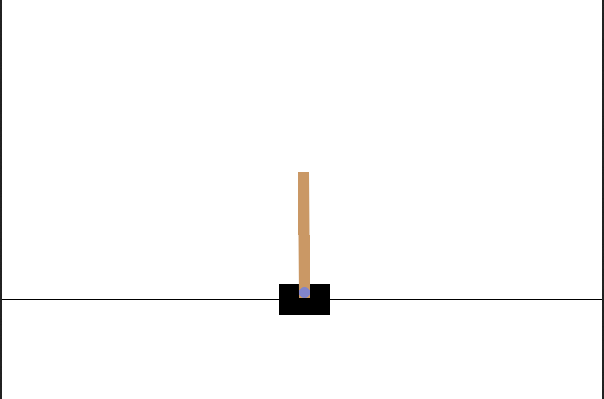
\includegraphics[width=0.6\textwidth]{./images/cartpole.png}
    
    \caption{Вид среды CartPole.}
    \label{fig:cartpole_scheme}
\end{figure}

\subsubsection{Пространство состояний}

Сенсорный аппарат агента крайне ограничен. В каждый момент времени t среда передает агенту вектор $S_t$, состоящий ровно из 4 непрерывных кинематических значений:

\begin{itemize}

  \item Позиция каретки: Текущее положение тележки на треке (от $-4.8$ до $4.8$ условных единиц). Такие значения обусловлены тем, что в оригинальном физическом эксперименте длина направляющего трека, по которому ездит тележка, составляла ровно 4.8 метра. Поскольку начальная позиция тележки находится ровно посередине трека, физический предел движения влево и вправо составляет ровно $\pm2.4$ метра. Этот предел был увеличен в два раза для того, чтобы среда успела зафиксировать окончательные значения при выходе агента за границы среды.
  \item Скорость каретки: Линейная скорость перемещения тележки.
  \item Угол отклонения шеста: Текущий угол наклона маятника относительно идеальной вертикали (в радианах).
  \item Угловая скорость шеста: Скорость падения или выравнивания маятника.

\end{itemize}

Именно этот вектор подается на входные узлы нейронной сети в процессе оценки приспособленности.

\subsubsection{Пространство действий}

Пространство возможных решений агента дискретно. На каждом шаге агент обязан выдать одну из двух команд:

\begin{itemize}
  
  \item 0: приложить фиксированный импульс силы, толкнув каретку влево.  
  \item 1: приложить фиксированный импульс силы, толкнув каретку вправо.

\end{itemize}

Важной особенностью является отсутствие действия «ничего не делать». Агент вынужден постоянно совершать микрокорректировки, что требует от нейросети быстрой реакции и точного балансирования между противоположными командами.

\subsubsection{Функция награды и условия завершения}

Награда в этой среде максимально проста: агент получает +1 за каждый такт времени, в течение которого шест остается в допустимом вертикальном положении.

Эпизод симуляции считается завершенным при выполнении любого из следующих условий:

\begin{enumerate}

  \item Падение: Угол отклонения шеста $\theta$ превысил допустимый порог (как правило, $\pm12^{\circ}$ или $\approx0.2095$ радиан от вертикали). Это ограничение основано на линейном приближении синуса малых углов.
  \item Выход за границы: Каретка уехала слишком далеко от центра экрана (позиция $x < -2.4$ или $x > 2.4$).
  \item Успех: Достигнут лимит времени симуляции (в версии среды CartPole-v1 этот лимит составляет 500 шагов).

\end{enumerate}

Агент должен достичь значения функции приспособленности в 500. Это означает, что нейросеть агента сформировала устойчивую стратегию балансировки, способную в рамках лимита среды поддерживать равновесие.

\subsubsection{Конфигурация алгоритма NEAT для среды CartPole}

Ниже приведены ключевые параметры, которые мы использовали в экспериментах:

\paragraph{Начальная топология и архитектура}

В соответствии с принципом постепенного усложнения структуры мы инициировали топологию нейросети с минимально возможной. Сеть не содержала скрытых слоев (num\_hidden = 0). Входной слой состоял из 4 нейронов, принимающих вектор состояния среды: позицию каретки, ее линейную скорость, угол отклонения шеста от вертикали и его угловую скорость. Выходной слой включал 2 нейрона, аппроксимирующих уверенность агента в необходимости приложения силы влево или вправо.

На старте эволюции мы применили также полную связность прямого распространения (initial\_connection = full\_direct). Выбор итогового дискретного действия агента осуществлялся путем вычисления максимума аргумента по вектору выходных значений сети. В качестве базовой функции активации для узлов применялась функция ReLU (activation\_default = relu).


\paragraph{Параметрические и структурные мутации:}

В процессе настройки \href{https://github.com/Isn0v/neat-training/blob/master/environments/cartpole/neat/neat.cfg}{конфигурационного файла}\footnote{\url{https://github.com/Isn0v/neat-training/blob/master/environments/cartpole/neat/neat.cfg}} мы намеренно сместили фокус на активную параметрическую адаптацию. На практике это работало так: алгоритм с высокой вероятностью (80\%, параметр weight\_mutate\_rate = 0.8) корректировал веса уже существующих связей, однако сама амплитуда этих изменений жестко сдерживалась параметром weight\_mutate\_power = 0.5.

Что касается структурного роста сети, мы решили отдать приоритет уплотнению связей, а не генерации новых узлов. Логика здесь проста: алгоритм должен по максимуму выработать потенциал текущей размерности графа, прежде чем наращивать его вычислительную сложность. Именно поэтому шанс образования нового синапса составил 50\% (conn\_add\_prob = 0.5), тогда как внедрение дополнительного скрытого нейрона допускалось значительно реже — лишь с вероятностью 20\% (node\_add\_prob = 0.2).

\paragraph{Параметры популяции и критерии сходимости:}

Размер эволюционирующей популяции мы задали на уровне 50 особей в каждом поколении (pop\_size = 50). Оценка приспособленности заключалась в суммарной награде, получаемой агентом за удержание маятника без падения и выхода за границы допустимой зоны.

В качестве критерия раннего останова и успешного завершения обучения мы установили порог приспособленности fitness\_threshold = 500, что соответствует максимально возможной оценке в стандартной спецификации среды CartPole-v1. Максимальный горизонт эволюции был ограничен 50 поколениями, однако, как показали дальнейшие эксперименты, алгоритм успешно находил оптимальную топологию задолго до исчерпания этого лимита.


\subsubsection{Архитектура и гиперпараметры агента DQN для среды CartPole}

Программная реализация алгоритма Deep Q-Network выполнялась с использованием библиотеки глубокого обучения PyTorch.

\paragraph{Архитектура нейронной сети:}

Чтобы аппроксимировать функцию ценности действий, мы спроектировали максимально компактную полносвязную сеть прямого распространения. На вход подается вектор из четырех элементов, описывающий текущую кинематику системы: координаты и скорости каретки, а также самого шеста. 

Скрытый слой мы намеренно ограничили всего 16 нейронами с функцией активации ReLU, потому что пространство состояний в среде CartPole-v1 довольно простое, и небольшая размерность сети не только спасает модель от переобучения, но и ощутимо ускоряет вычислительные проходы прямого и обратного распространения ошибки. На выходе формируются сигналы от двух нейронов с линейной активацией — они выдают предсказанные Q-значения для каждого из доступных действий (толчок влево или вправо). Итоговое решение агент принимает, просто выбирая аргумент максимального значения из этого вектора. 


\paragraph{Стратегия исследования и дисконтирование:}

Для соблюдения баланса между исследованием среды и эксплуатацией уже проверенных стратегий мы опирались на классическую $\epsilon$-жадную политику. На старте параметр исследования был выставлен в максимальное значение, равное 1. По мере обучения доля случайных действий плавно срезалась: на каждом шаге применялся коэффициент затухания $\epsilon_{decay} = 0.995$, пока исследование не упиралось в минимальный порог $\epsilon_{min} = 0.01$. Дополнительно мы задали высокий фактор дисконтирования ($\gamma = 0.99$). Он обеспечивал алгоритму необходимую «дальновидность», заставляя придавать огромный вес будущим потенциальным наградам, что является критическим условием для долгосрочной балансировки маятника.


\paragraph{Буфер памяти и процесс оптимизации:}

Для стабилизации процесса обучения нейронной сети использовался механизм воспроизведения опыта. Взаимодействия агента со средой сохранялись в циклический буфер памяти емкостью 10 000 переходов. На каждом шаге обучения (после накопления достаточного объема данных) из буфера случайным образом сэмплировался мини-батч размером 64 перехода. Это позволило разорвать временную корреляцию между последовательными состояниями и свести к минимуму дисперсию градиентов при обновлении весов.

Обновление весовых коэффициентов сети осуществлялось с помощью оптимизатора Adam со скоростью обучения 0.001. В качестве целевой метрики использовалась среднеквадратичная ошибка. Минимизируемая функция потерь $L$ строилась на основе отклонения текущего предсказания сети от целевого значения, вычисляемого согласно уравнению Беллмана:

\begin{equation}
  \label{eq:dqn_loss}
  L = \frac{1}{N} \sum_{t=0}^{T} ((r_t + \gamma \underset{a'}{max} Q(s_{t}, a')) - Q(s_t, a_t))^2
\end{equation}

где $N$ -- размер батча, $s_t$ и $a_t$ -- текущие состояние и действие, $r_t$ -- полученная награда, $s'_t$ -- следующее состояние, а $\gamma$ -- коэффициент дисконтирования.

Критерием успешного решения среды служило достижение суммарной награды в 500 баллов за один эпизод, что означает непрерывное удержание шеста в течение 500 тактов симуляции. По достижении этого порога веса модели (state\_dict) автоматически сохранялись для последующей демонстрации и анализа.

\subsection{Среда LunarLander}

Среда LunarLander впервые упоминается в пакете сред Gym \cite{towers2025gymnasiumstandardinterfacereinforcement}, которая представляет собой задачу управления в условиях двумерной физической симуляции с непрерывным пространством состояний. Задача когнитивного агента заключается в осуществлении безопасной и мягкой посадки космического модуля на заданную посадочную площадку, расположенную между двумя маркерными флажками. В отличие от задачи балансировки маятника, здесь агент должен научиться преодолевать гравитацию и управлять инерцией, аккуратно дозируя тягу главного и двух маневровых двигателей.

В рамках данного исследования для оценки способности алгоритмов к обобщению устойчивости тестирование проводилось в двух различных конфигурациях среды: в условиях идеального вакуума и с применением сильного бокового ветра и турбулентности. Сравнительный анализ влияния этих возмущающих факторов на стабильность агентов подробно рассматривается в разделе экспериментальных результатов.

\begin{figure}[h!] % [h!] - попытка разместить картинку "здесь" (here)
  \centering
  
  % 0.7 от ширины текста страницы (0.7\textwidth)
  % Замени 'cartpole_env.png' на реальное имя твоего файла, если оно другое.
  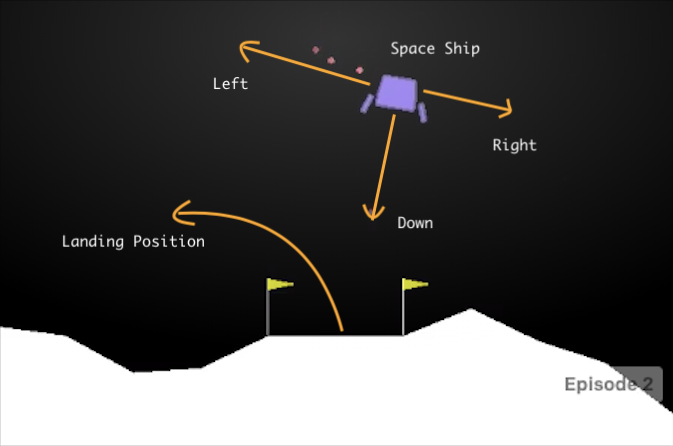
\includegraphics[width=0.6\textwidth]{./images/lunarlander.png}
  
  \caption{Вид среды LunarLander.}
  \label{fig:lunarlander_scheme}
\end{figure}


\subsubsection{Пространство состояний}

Сенсорный аппарат агента передает вектор наблюдений, состоящий из 8 числовых параметров, исчерпывающе описывающих текущее кинематическое состояние модуля:

\begin{itemize}

  \item \textbf{Позиция центра масс} аппарата в двумерной системе координат ($x, y$).

  \item \textbf{Вектор линейной скорости} перемещения модуля по осям $x$ и $y$.

  \item \textbf{Угол наклона (крена)} аппарата относительно идеальной вертикали.

  \item \textbf{Угловая скорость} вращения модуля.

  \item \textbf{Два дискретных булевых флага}, сигнализирующих о наличии физического контакта левой и правой посадочных опор с поверхностью.

\end{itemize}

\subsubsection{Пространство действий}

Пространство возможных решений агента является дискретным и состоит из 4 взаимоисключающих команд, выбираемых нейросетью на каждом такте симуляции:

\begin{itemize}

  \item \textbf{0:} Не предпринимать никаких действий (свободное падение).

  \item \textbf{1:} Включить левый маневровый двигатель (для корректировки крена вправо).

  \item \textbf{2:} Включить главный (нижний) маршевый двигатель.

  \item \textbf{3:} Включить правый маневровый двигатель (для корректировки крена влево).

\end{itemize}

\subsubsection{Функция награды и условия завершения}

В отличие от бинарного сигнала выживания в CartPole, функция приспособленности в LunarLander имеет сложную композитную структуру, стимулирующую достижение цели при максимальной экономии ресурсов:

\begin{itemize}

  \item За успешное касание поверхности обеими опорами агенту начисляется бонус в +100 очков.

  \item За движение к центру целевой площадки и корректное снижение скорости присуждается от +100 до +140 очков.

  \item В случае крушения модуля (падения на корпус) накладывается строгий штраф в размере -100 очков.

  \item Работа двигателей пенализируется для оптимизации расхода топлива: каждый такт работы главного двигателя стоит -0.3 очка , а использование боковых маневровых двигателей штрафуется на -0.03 очка за такт.

\end{itemize}

Один эпизод симуляции принудительно обрывается при достижении лимита в 1000 шагов, а также при успешной посадке или крушении модуля. Идеальная, мягкая посадка в центр площадки позволяет набрать около 250–300 очков. Официальным порогом успешного решения среды, свидетельствующим о сходимости алгоритма, считается достижение средней награды в 200 баллов.

\subsubsection{Конфигурация алгоритма NEAT для LunarLander}

\href{https://github.com/Isn0v/neat-training/blob/master/environments/lunar-lander/neat/neat.cfg}{Файл конфигурации NEAT}\footnote{\url{https://github.com/Isn0v/neat-training/blob/master/environments/lunar-lander/neat/neat.cfg}} определяет фундаментальные правила эволюции. Ниже приведены ключевые параметры, использованные в экспериментах:


\paragraph{Основные параметры популяции и завершения:}
  \begin{itemize}

    \item \textbf{Размер популяции (pop\_size = 150):} Данный параметр устанавливает количество нейронных сетей в каждом поколении. Значение 150 выбрано для обеспечения достаточного разнообразия геномов и эффективного поиска в пространстве решений.

    \item \textbf{Критерий приспособленности (fitness\_criterion = max):} Эволюция стремится максимизировать функцию приспособленности, выбирая лучшие геномы для размножения.

    \item \textbf{Порог приспособленности (fitness\_threshold = 200.0):} Обучение считается завершенным, если хотя бы один агент набирает 200.0 очков (стандартный порог решения среды).

  \end{itemize}

\paragraph{Архитектура и инициализация генома:}

  \begin{itemize}

    \item \textbf{Входы и Выходы:} Количество входных нейронов (num\_inputs = 8) и выходных нейронов (num\_outputs = 4) жестко зафиксировано и соответствует спецификации среды LunarLander.

    \item \textbf{Начальные скрытые слои (num\_hidden = 0):} Поиск начинается с самых простых сетей, без скрытых нейронов, чтобы позволить алгоритму NEAT самостоятельно развить сложную топологию.

    \item \textbf{Функции активации (activation\_default = tanh):} Все нейроны используют функцию активации гиперболического тангенса, которая позволяет вводить нелинейность в работу сети и выдает значения в диапазоне [-1, 1], что подходит для управления двигателями.

    \item \textbf{Начальные связи (initial\_connection = full\_direct):} На старте каждый входной нейрон соединен со всеми выходными нейронами, что обеспечивает минимальную функциональность сети.

  \end{itemize}

\paragraph{Вероятности мутации:}
  \begin{itemize}

    \item \textbf{Мутация весов (weight\_mutate\_rate = 0.8):} С вероятностью 80\% вес существующей связи будет изменен. Высокое значение стимулирует постоянное уточнение "тонкой настройки" управления.

    \item \textbf{Добавление нейрона/связи (node\_add\_prob = 0.2, conn\_add\_prob = 0.5):} Задают вероятности добавления нового скрытого нейрона (20\%) или новой синаптической связи (50\%). Это обеспечивает рост сложности топологии сети.

    \item \textbf{Удаление нейрона/связи (node\_delete\_prob = 0.2, conn\_delete\_prob = 0.5):} Задают вероятности удаления нейронов или связей, что позволяет упрощать избыточные структуры.

  \end{itemize}

\paragraph{Специация и эволюция популяции:}
  \begin{itemize}

    \item \textbf{Видообразование (compatibility\_threshold = 3.0):} Порог совместимости $\delta$ в 3.0 очка определяет, насколько генетически различными должны быть сети, чтобы считаться разными видами.

    \item \textbf{Застой видов (max\_stagnation = 20):} Если лучшая приспособленность вида не улучшается в течение 20 поколений, он считается застойным и не получает ресурсов для размножения. Это предотвращает "зацикливание" эволюции на локальных максимумах.

    \item \textbf{Элитизм (species\_elitism = 2):} Два лучших вида популяции защищены от удаления даже при застое.

    \item \textbf{Воспроизводство (elitism = 2, survival\_threshold = 0.2):} В каждом виде два лучших генома гарантированно выживают, и только 20\% наиболее приспособленных особей вида получают право на размножение.

  \end{itemize}


\subsubsection{Архитектура и гиперпараметры агента DQN для среды LunarLander}

Программная реализация алгоритма DQN для задачи посадки лунного модуля базировалась на фреймворке \texttt{stable\_baselines3}, рассмотренном в работе \cite{stable_baselines3}. Он предоставляет оптимизированные и надежные реализации современных алгоритмов обучения с подкреплением. В связи с необходимостью комплексной оценки устойчивости когнитивных агентов, обучение проводилось в два этапа: формирование \href{https://github.com/Isn0v/neat-training/blob/master/environments/lunar-lander/rl/model.py}{базовой политики управления}\footnote{\url{https://github.com/Isn0v/neat-training/blob/master/environments/lunar-lander/rl/model.py}} и \href{https://github.com/Isn0v/neat-training/blob/master/environments/lunar-lander/rl/model_windy.py}{универсальной политики}\footnote{\url{https://github.com/Isn0v/neat-training/blob/master/environments/lunar-lander/rl/model_windy.py}} в условиях ветренности.

Процесс Q-обучения регулировался следующим набором гиперпараметров:

\begin{itemize}

  \item \textbf{Буфер воспроизведения опыта:} Емкость буфера составила 100 000 переходов, что обеспечило эффективную декорреляцию обучающей выборки. Процесс обучения инициировался после накопления первых 1 000 случайных шагов (learning\_starts = 1000).

  \item \textbf{Оптимизация и градиентный спуск:} Использовался размер пакета данных равный 128. Скорость обучения была установлена на уровне $10^{-3}$.

  \item \textbf{Параметры обновления:} Дисконтирующий множитель $\gamma$ составил 0.99, ориентируя агента на долгосрочное планирование. Синхронизация весов целевой сети производилась каждые 250 шагов оптимизации.

  \item \textbf{Стратегия исследования среды:} Применялась $\epsilon$-жадная стратегия с линейным затуханием. Начальное значение параметра исследования $\epsilon = 1.0$ постепенно снижалось до $0.05$ на протяжении первых 10\% от общего времени обучения (exploration\_fraction = 0.1), после чего агент переходил к преимущественной эксплуатации полученных знаний.

\end{itemize}


\subsection{Среда Ant}

В качестве полигона для исследования возможностей нейроэволюции была выбрана среда непрерывного управления Ant-v4 из библиотеки Gymnasium. Данная среда представляет собой физическую симуляцию на базе движка MuJoCo, описанную в \cite{mujoco}, для четырехногого агента («муравья»), цель которого -- максимально быстро и эффективно продвигаться вперед (по оси X), сохраняя при этом баланс и минимизируя затраты энергии на лишние движения.

\begin{figure}[h!]
  \centering
  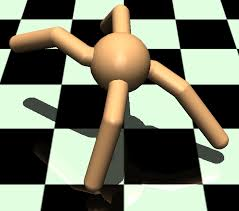
\includegraphics[width=0.6\textwidth]{./images/ant.png}
  \caption{Схематическое изображение агента в среде Ant-v4.}
  \label{fig:ant}
\end{figure}

\subsubsection{Пространство состояний и действий}

Сложность среды обусловлена физическими параметрами модели:

\begin{itemize}

  \item Пространство состояний (27 параметров): включает в себя данные о положении корпуса в пространстве, углы поворота всех восьми сочленений, а также векторы их линейных и угловых скоростей. Такой объем данных необходим нейросети для понимания текущей позы робота и инерции его частей.

  \item Пространство действий (8 параметров): агент управляет крутящими моментами, прикладываемыми к каждому из восьми суставов. Действия являются непрерывными и лежат в диапазоне $[-1, 1]$.
\end{itemize}

\subsubsection{Функция награды и условия завершения}

Функция приспособленности в данном эксперименте базируется на стандартной системе вознаграждений Ant-v4, которая включает:

\begin{enumerate}

  \item Reward for moving forward: поощрение за продвижение вдоль оси X.

  \item Healthy reward: фиксированный бонус за каждый шаг, пока робот остается «здоров» (не перевернулся и не вышел за пределы допустимых углов).

  \item Control cost: штраф за слишком резкие или энергозатратные движения, что стимулирует агента к плавной и естественной походке.

\end{enumerate}

Для оптимизации процесса эволюции была внедрена эвристика «жесткого таймера». Если в течение 50 шагов симуляции агент не продвигается вперед более чем на 0.05 метра, эпизод прерывается досрочно. Это позволяет алгоритму быстрее переходить к оценке следующей особи, не тратя время на агентов, которые застряли или совершают хаотичные движения на месте. Окончательная оценка генома вычисляется как среднее арифметическое результатов трех независимых эпизодов.

\subsubsection{Конфигурация алгоритма NEAT для среды Ant-v4}


\href{https://github.com/Isn0v/neat-training/blob/master/environments/ant/neat.cfg}{Настройка}\footnote{\url{https://github.com/Isn0v/neat-training/blob/master/environments/ant/neat.cfg}} алгоритма NEAT для среды Ant-v4 оказалась непростой задачей. Главная сложность заключалась в высокой размерности пространства действий: малейшие хаотичные скачки в топологии растущей сети могли легко разрушить только начавший формироваться навык ходьбы агента. Чтобы взять этот процесс под контроль, мы разделили архитектуру решения на три обособленных блока: базовые архитектурные параметры, генетические механизмы и саму вычислительную инфраструктуру.

\paragraph{Архитектурные параметры и инициализация:}

Стартовую архитектуру нейросетей мы также сделали примитивной. Размерность слоев мы жестко привязали к физической модели «муравья»: сеть получила 27 сенсорных узлов на входе и 8 моторных на выходе.

Как и в предыдущих экспериментах, мы полностью отказались от использования скрытых нейронов на старте. Все сенсорные данные напрямую пробрасывались на выходы. Подобный подход давал эволюции возможность сперва отточить базовые линейные зависимости в управлении роботом, и лишь затем, по мере необходимости, выстраивать сложные нелинейные цепи.

Для выходных сигналов идеально подошел гиперболический тангенс, потому что он совпадает с требованиями физического движка MuJoCo к управляющим импульсам. При этом классическое суммирование входящих сигналов внутри узлов мы заменили на усреднение.

\paragraph{Генетические операторы и мутации:}

\begin{itemize}

  \item Генетические операторы: Для обеспечения баланса между эксплуатацией текущих решений и исследованием новых топологий были установлены следующие коэффициенты:

  \item Мутация весов и смещений: используется гауссово распределение со средним значением 0.0 и стандартным отклонением 0.1. Максимальные и минимальные значения весов ограничены диапазоном $[-3.0, 3.0]$ для предотвращения «взрыва» активаций в глубоких слоях эволюционирующей сети.

  \item Структурные мутации: вероятность добавления новой связи (conn\_add\_prob) составляет 0.3, а добавления нового узла (node\_add\_prob) -- 0.1. При этом вероятности удаления компонентов (conn\_delete\_prob, node\_delete\_prob) установлены в 0, что гарантирует сохранение накопленной сложности топологии в рамках данного эксперимента. Данное решение было принято для ускорения сходимости, так как большинство полезных мутаций в Ant-v4 связано с добавлением новых связей, а не удалением существующих.

\end{itemize}

\paragraph{Видообразование и репродукция:}

Порог генетической совместимости был зафиксирован на отметке 1.2. На практике это позволило аккуратно дробить обширную популяцию из 500 особей на изолированные, устойчивые группы с похожими топологиями сетей. Внутри каждого сформированного вида гарантированно выживала только одна лучшая особь, тогда как для популяции в целом этот лимит составлял 5 агентов, набравших наибольший результат приспособленности. Право участвовать в кроссинговере и передавать свои гены следующему поколению получали лишь 20\% наиболее результативных агентов.

\paragraph{Инфраструктура обучения и отказоустойчивость:}

Перейдем к технической реализация, находящейся в файле \href{https://github.com/Isn0v/neat-training/blob/master/environments/ant/model.py}{model.py}\footnote{\url{https://github.com/Isn0v/neat-training/blob/master/environments/ant/model.py}}.

Вычисления в среде Ant-v4 ресурсоемки, поэтому нам пришлось внедрить ряд решений для обеспечения стабильности экспериментов.  Во-первых, мы ушли от последовательного выполнения кода и распределили расчет приспособленности агентов на все доступные ядра процессора с помощью инструмента ParallelEvaluator. Такая параллелизация позволила радикально ускорить симуляцию, сократив время обработки одного поколения примерно в 4–8 раз в соответствии с количеством физических ядер устройства.  Во-вторых, мы учли тот факт, что эволюция многосуставного робота — это тяжелый процесс, который может длиться от нескольких часов до нескольких дней. В таких условиях очень важной оказалась отказоустойчивость. Мы настроили систему чекпоинтов и теперь алгоритм автоматически делает полный срез популяции и сохраняет весь накопленный прогресс каждые 25 поколений. Это надежно страховало нас от потери результатов в случае любых системных сбоев или переполнения памяти. 